\documentclass[tikz,border=8pt]{standalone}
% Shared look for every TikZ diagram. Load with \input{../../tools/tikz-style.tex}
\usepackage[T1]{fontenc}
\usepackage{lmodern}
\renewcommand{\sfdefault}{lmr}  % diagrams use the same serif as the text
\usetikzlibrary{arrows.meta, positioning, shapes.geometric, calc, fit, backgrounds}
\definecolor{cblue}{HTML}{4C78A8}
\definecolor{corange}{HTML}{F58518}
\definecolor{cgreen}{HTML}{54A24B}
\definecolor{cred}{HTML}{E45756}
\definecolor{cpurple}{HTML}{B279A2}
\definecolor{cgrey}{HTML}{6B6B6B}
\tikzset{
  every picture/.style={font=\sffamily, line width=1.2pt},
  box/.style={draw=#1, fill=#1!12, rounded corners=4pt, align=center, inner sep=7pt, minimum height=1.1cm},
  box/.default=cgrey,
  arrow/.style={-{Stealth[length=3mm]}, draw=cgrey, line width=1.4pt},
  title/.style={font=\sffamily\bfseries\Large},
  note/.style={font=\sffamily\small, text=cgrey, align=center},
}
\AtBeginDocument{\hyphenpenalty=10000 \exhyphenpenalty=10000}

\begin{document}
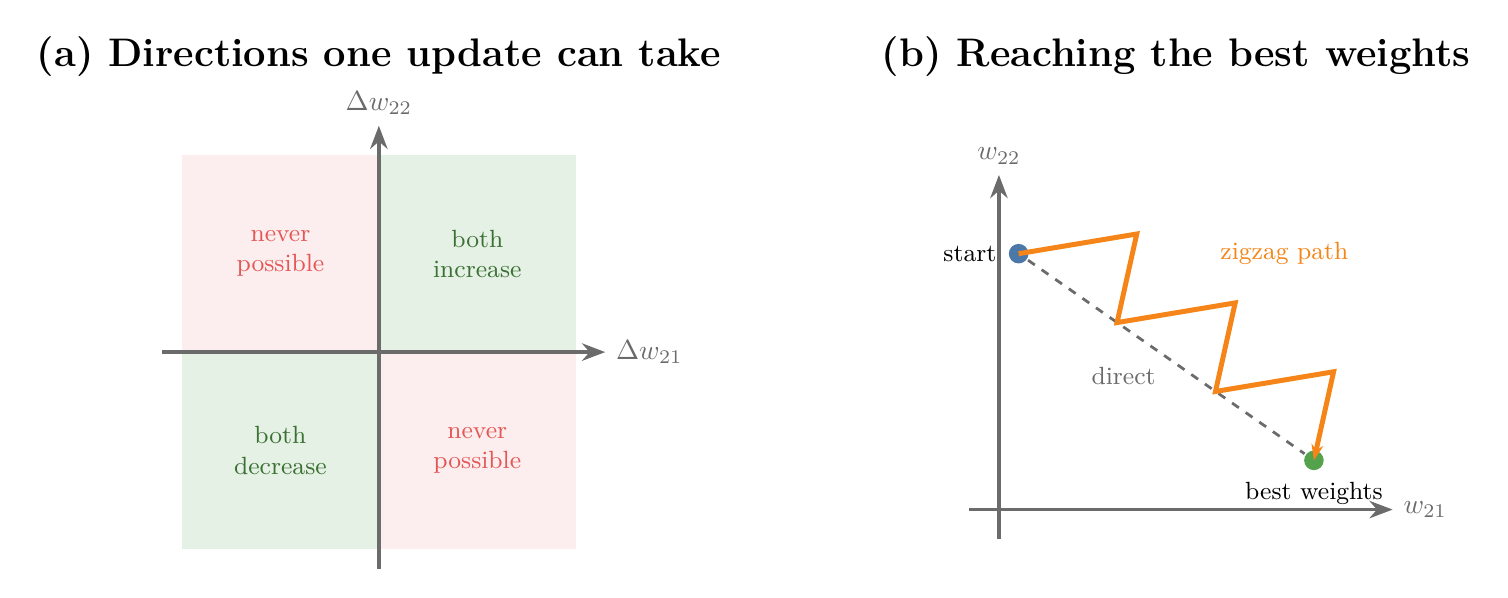
\begin{tikzpicture}[scale=1.25]
  % (a) allowed directions
  \begin{scope}
    \fill[cgreen!15] (0,0) rectangle (2,2);
    \fill[cgreen!15] (0,0) rectangle (-2,-2);
    \fill[cred!10] (0,0) rectangle (2,-2);
    \fill[cred!10] (0,0) rectangle (-2,2);
    \draw[cgrey, -{Stealth}] (-2.2,0) -- (2.3,0) node[right] {$\Delta w_{21}$};
    \draw[cgrey, -{Stealth}] (0,-2.2) -- (0,2.3) node[above] {$\Delta w_{22}$};
    \node[font=\sffamily\small, text=cgreen!70!black, align=center] at (1,1) {both\\increase};
    \node[font=\sffamily\small, text=cgreen!70!black, align=center] at (-1,-1) {both\\decrease};
    \node[font=\sffamily\small, text=cred, align=center] at (1,-1) {never\\possible};
    \node[font=\sffamily\small, text=cred, align=center] at (-1,1) {never\\possible};
    \node[title] at (0,3.0) {(a) Directions one update can take};
  \end{scope}
  % (b) zigzag path
  \begin{scope}[xshift=6.3cm, yshift=-1.6cm]
    \draw[cgrey, -{Stealth}] (-0.3,0) -- (4.0,0) node[right] {$w_{21}$};
    \draw[cgrey, -{Stealth}] (0,-0.3) -- (0,3.4) node[above] {$w_{22}$};
    \node[circle, fill=cblue, inner sep=2.5pt, label={[font=\sffamily\small]left:start}] (s) at (0.2,2.6) {};
    \node[circle, fill=cgreen, inner sep=2.5pt, label={[font=\sffamily\small]below:best weights}] (t) at (3.2,0.5) {};
    \draw[cgrey, dashed, line width=1pt] (s) -- (t) node[midway, below left, font=\sffamily\small] {direct};
    \draw[corange, line width=1.8pt, -{Stealth[length=2mm]}]
      (0.2,2.6) -- ++(1.2,0.2) -- ++(-0.2,-0.9) -- ++(1.2,0.2) -- ++(-0.2,-0.9) -- ++(1.2,0.2) -- ++(-0.2,-0.9);
    \node[font=\sffamily\small, text=corange] at (2.9,2.6) {zigzag path};
    \node[title] at (1.8,4.6) {(b) Reaching the best weights};
  \end{scope}
\end{tikzpicture}
\end{document}
